\begin{frame}[parent={cmap:software-testing},hasnext=true,hasprev=true]
\label{concept:softwar-testing:process}
\frametitle{Software testing process}

\begin{block:fact}{Software testing process}
\begin{itemize}
	\item When conducted in a systematic and clear-sighted way, software
	testing helps to:
	\begin{itemize}
		\item Increase confidence that the product behaves according to its
		specification.

		\item Highlight minimal characteristics of product quality.
	\end{itemize}
\end{itemize}
\end{block:fact}

\begin{block:fact}{}
\end{block:fact}
\end{frame}


\begin{frame}[parent={cmap:software-testing},hasnext=false,hasprev=true]
\frametitle{Software testing concepts}
\framesubtitle{Software testing}

\begin{figure}
	\centering
	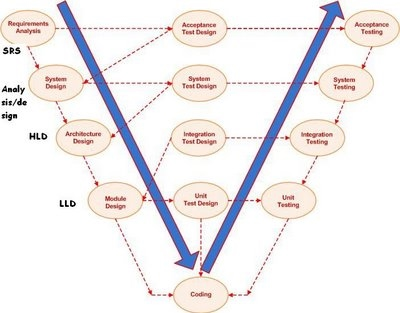
\includegraphics[width=8cm]{v-model}
\end{figure}
\end{frame}